\documentclass[a4paper,11pt]{report}

\usepackage{amsmath,amssymb}
\usepackage{fullpage}
\usepackage{graphicx}
\usepackage[cache=false]{minted}

\usepackage{bussproofs}
\usepackage{mathpartir}
\usepackage{prooftrees}
\usepackage{color}

\usepackage{tikz}
\usetikzlibrary{automata,positioning}

\newcommand*\circled[1]{\tikz[baseline=(char.base)]{
    \node[shape=circle,draw,inner sep=2pt] (char) {#1};}}

\makeatletter
\pgfmathdeclarefunction{alpha}{1}{%
  \pgfmathint@{#1}%
  \edef\pgfmathresult{\pgffor@alpha{\pgfmathresult}}%
}

\newcommand*{\until}{U}
\newcommand*{\disj}{\ ,\ }
\newcommand*{\A}{\square}  % Always
\newcommand*{\D}{\diamondsuit} % eventually

\newcommand*{\Pq}{(\top,\bot)}
\newcommand*{\pQ}{(\bot,\top)}
\newcommand*{\PQ}{(\top,\top)}
\newcommand*{\pq}{(\bot,\bot)}

\usemintedstyle{tango}

\newminted[promelacode]{C}{
  frame=single,
  framesep=6pt,
  breaklines=true,
  fontsize=\scriptsize
}

\newmintinline[promelainline]{C}{breaklines=true,fontsize=\small}

\newmintedfile{c}{frame=single, framesep=6pt, breaklines=true,fontsize=\scriptsize}
\newcommand{\ex}[3]{\cfile[firstline=#1,lastline=#2]{ex#3.pml}}

% tikz
\usepackage{tikz}
\usetikzlibrary{snakes}

\author{Sylvain Julmy}
\date{\today}

\setlength{\parindent}{0pt}
\setlength{\parskip}{2.5pt}

\begin{document}

\begin{center}
  \Large{
    Verification of Cyber-Physical System\\
    Fall 2017
  }
  
  \noindent\makebox[\linewidth]{\rule{\linewidth}{0.4pt}}
  Exercice Sheet 7

  \vspace*{1.4cm}

  Author : Sylvain Julmy
  \noindent\makebox[\linewidth]{\rule{\linewidth}{0.4pt}}

  \begin{flushleft}
    Professor : Ultes-Nitsche Ulrich
    
    Assistant : Prisca Dotti
  \end{flushleft}

  \noindent\makebox[\linewidth]{\rule{\textwidth}{1pt}}
\end{center}

\section*{Exercice 1}

The two timed automaton from figures \ref{fig:processA} and \ref{fig:processB}
are an implementation with \texttt{UPPAAL} of the \texttt{Promela} model given
in exercice sheet :

\begin{figure}[h]
  \centering
  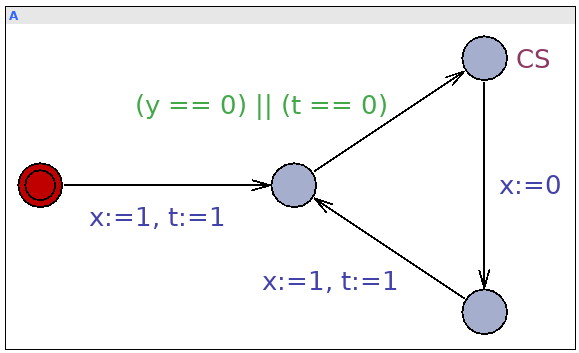
\includegraphics[width=0.6\textwidth]{figures/ex1_a}
  \caption{Process A}
  \label{fig:processA}
\end{figure}

\begin{figure}[h]
  \centering
  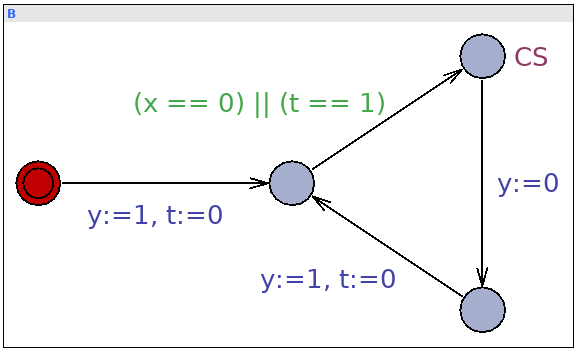
\includegraphics[width=0.6\textwidth]{figures/ex1_b}
  \caption{Process B}
  \label{fig:processB}
\end{figure}

Both process use the same concept and only the variable used are different. At
first, we start in an state that is unreachable from the other states of the
automaton, this state is used in order to initiliase the automaton variables.

The second state reached is representing the wait of a process, and only when
the corresponding property for each process holds, the transition can be taken.

The state named $CS$ is representing the critical section for each process, and
none of those can access the critical section at the same time.

The incoming state from $CS$ is representing the transition from \verb|x=false|
and \verb|x=true| in process $A$, we have to use such an additional state
because we have to represent the possibility that $B$ is making progress between
the two assignment \verb|x=false| and \verb|x=true| (the same holds for process
$B$ w.r.t. process $A$).

We also use the following declaration (listing \ref{lst:declaration}) and
composition (listing \ref{lst:composition}) for the system :

\begin{listing}[h]
  \centering
\begin{promelacode}
bool x,y,t;
\end{promelacode}
  \caption{Declarations}
  \label{lst:declaration}
\end{listing}

\begin{listing}[H]
\centering
\begin{promelacode}
// Place template instantiations here.
A = ProcessA();
B = ProcessB();
// List one or more processes to be composed into a system.
system A,B;
\end{promelacode}
\caption{Composition}
\label{lst:composition}
\end{listing}

In order to verify our system, we could use the verifier with the formula

\begin{verbatim}
A[] not(A.CS and B.CS)
\end{verbatim}

which verify that for all possible path (\verb|A|), this is always the case
(\verb|[]|) that \verb|A| and \verb|B| are not in the critical section at the
same time (\verb|p.CS| where \verb|p| is the corresponding process).

\section*{Exercice 2}

$x$ is a clock of the system, at each step, the clock would either be $0$ or
greater than $2$, the transition from $Idle$ to $Taken$ of process $B$ is taken
only when receiving something from chanel $reset$, then the only possible
transition after receiving something is the one from $Taken$ to $Idle$, where
the clock is reset.

The only constraint we have is that $x$ have to be greater or equals to $2$ in
order to send/receive from the $reset$ chanel.

Then, we want to modify the model in order to have the clock reset only when the
clock value is either $2$ or $3$.

\subsection*{Model proposition 1}

With the first proposition, we add the invariant $x \leq 3$ to the state
$loop$, so the system have to leave the state when $x \leq 3$ would become
$false$.

This proposition meet the requirement, because when $x$ would become higher than
$3$, the system is forced to leave the $Idle$ state and no deadlock is possible.

\subsection*{Model proposition 2}

With the second proposition, we modified the guard of the $reset$ send from $x
\geq 2$ to $x \geq 2\ \ \&\&\ \ x \leq 3$. It means that the clock can be reset
only if $x$ is between $2$ and $3$.

This proposition does not meet the requirement, because when $x$ would become
higher than $3$, the system is not forced to leave the $Idle$ state. If the
state is not leave, the system will entire in a deadlock because there is no
available transition.

\end{document}